\documentclass[../../../interview-questions.tex]{subfiles}

\begin{document}

\subsection{为什么Redis快}

Redis 的速度非常的快,单机的 Redis 就可以支撑每秒 10 几万的并发,相对于 MySQL 来说,性能是 MySQL(并发几百到几千)的几十倍。速度快的原因主要有几点:

\begin{enumerate}
    \item {\bf{基于内存}} 完全基于内存操作,Redis是基于内存存储实现的数据库,相对于数据存在磁盘的数据库,就省去磁盘磁盘I/O的消耗。
    \item {\bf{高效的数据结构}} C 语言实现,优化过的数据结构,基于几种基础的数据结构,Redis 做了大量的优化,性能极高。如简单动态字符串SDS、哈希、跳跃表、压缩列表ziplist。简单动态字符串SDS带来的好处就是以O(1)时间复杂度获取长度,在C语言中,要获取字符串的长度,需要从头开始遍历,复杂度为O(n)。减少内存重新分配的次数,在C语言中,修改一个字符串,需要重新分配内存,修改越频繁,内存分配就越频繁,而分配内存是会消耗性能的。而在Redis中,SDS提供了两种优化策略:空间预分配和惰性空间释放。为了保持高效,Redis 会对哈希表做rehash操作,也就是增加哈希桶,减少冲突。为了rehash更高效,Redis还默认使用了两个全局哈希表,一个用于当前使用,称为主哈希表,一个用于扩容,称为备用哈希表。

\begin{figure}[htbp]
    \centering
    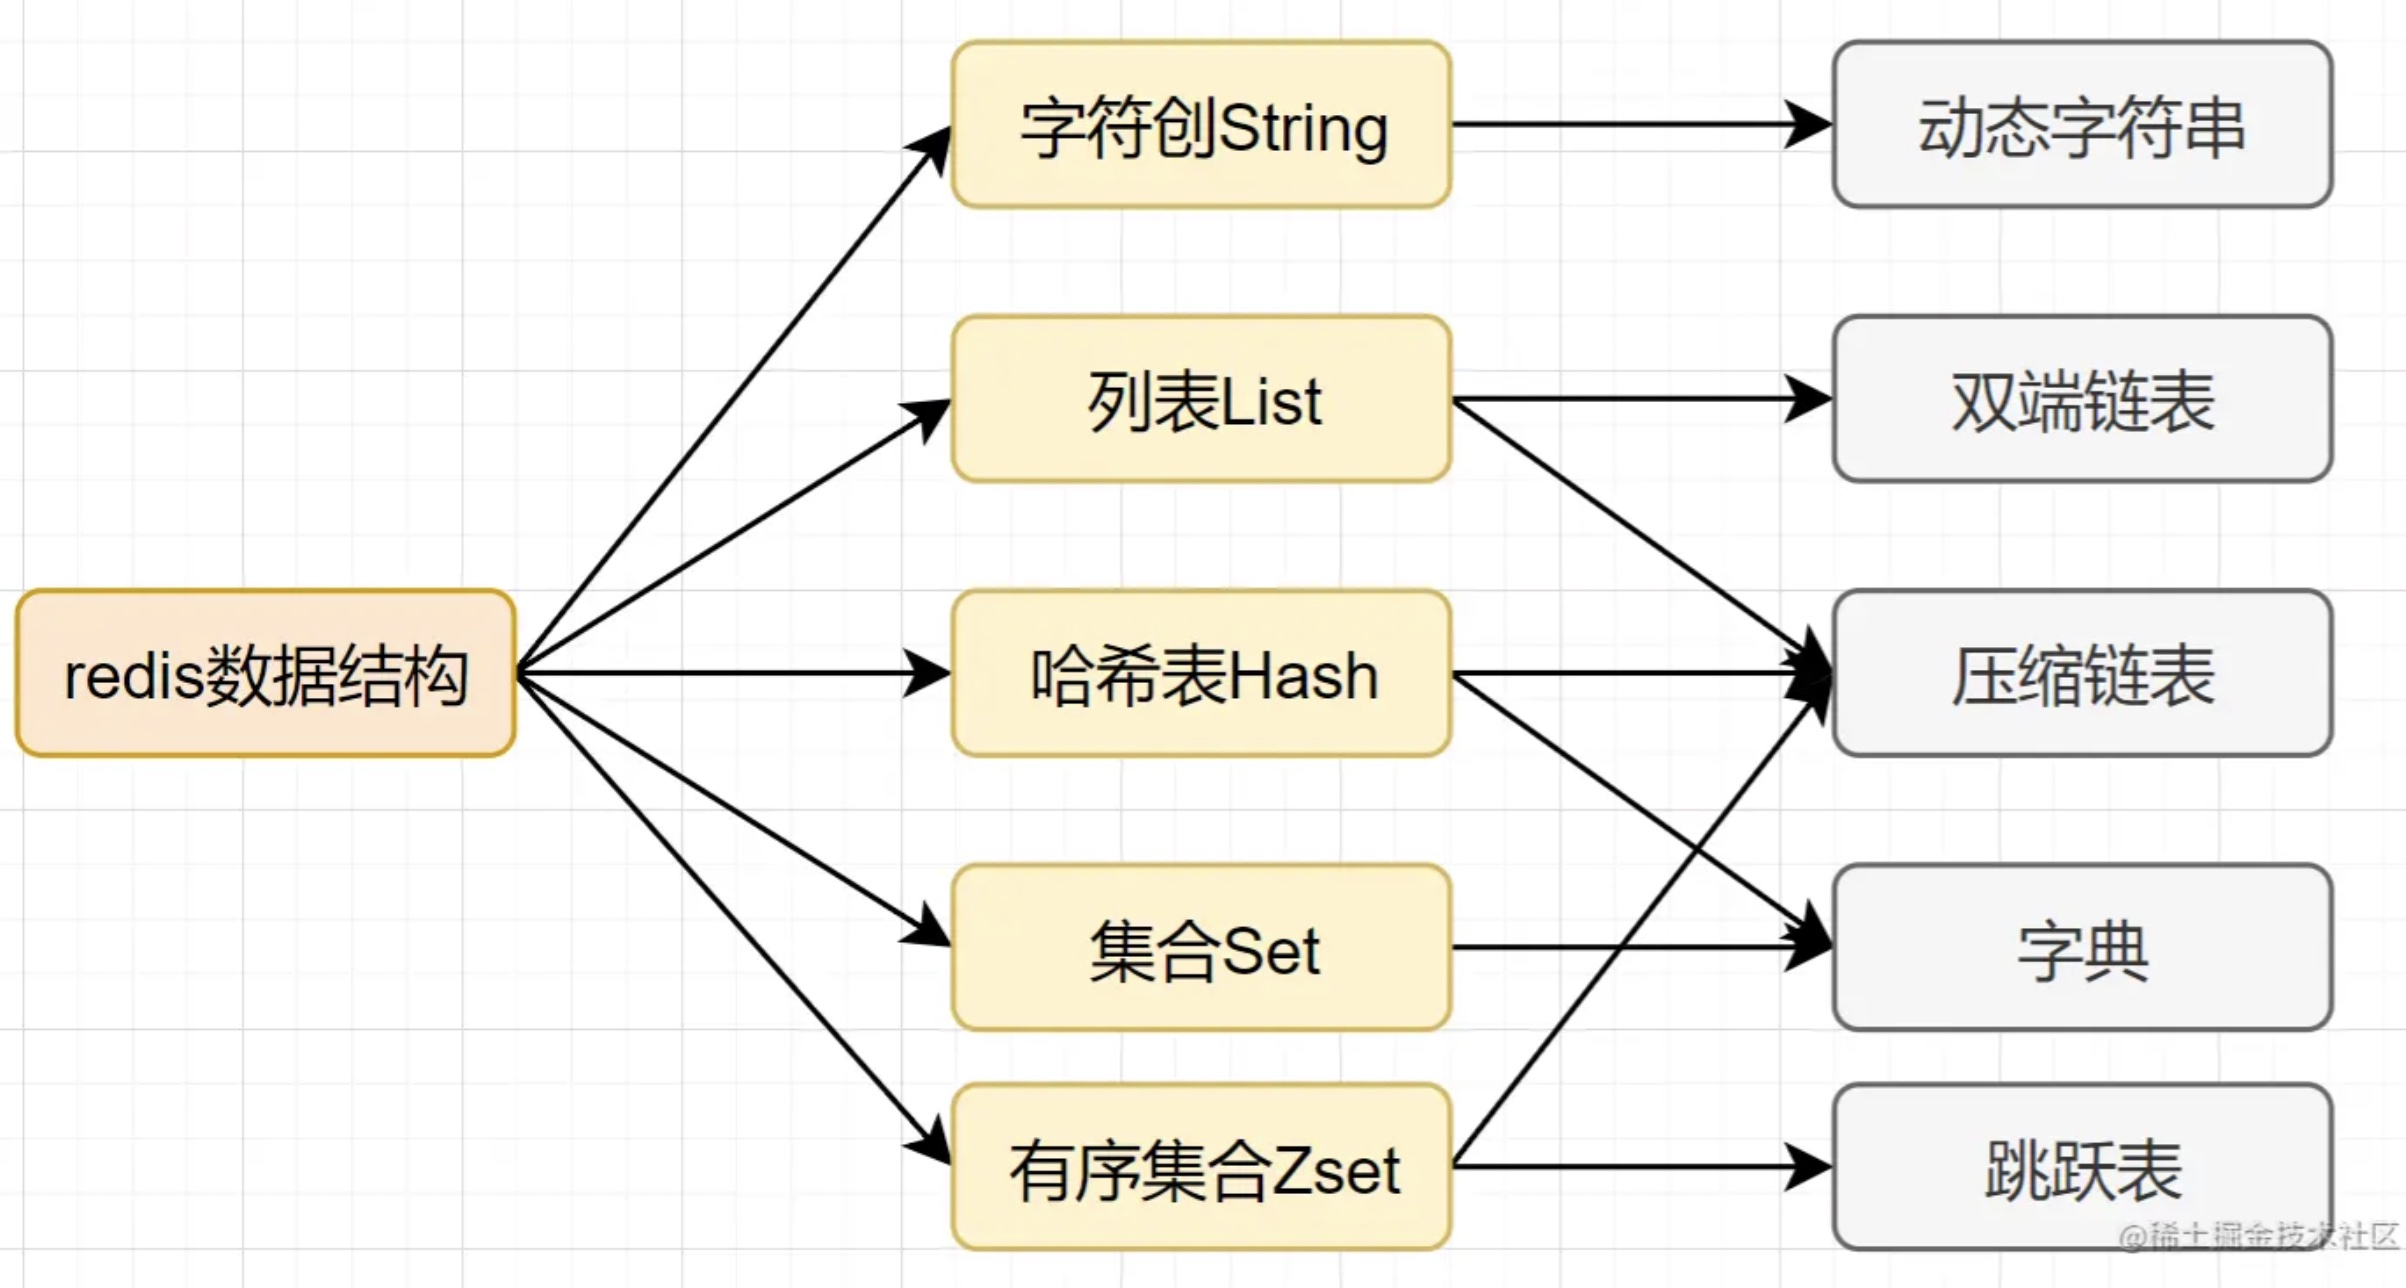
\includegraphics[scale=0.15]{redisdatastructure.jpg}
    \caption{Redis数据结构}
    \label{fig:redisdatastructure}
\end{figure}

    \item {\bf{合理的数据编码}}Redis支持多种数据基本类型,每种基本类型对应不同的数据结构,每种数据结构对应不一样的编码。为了提高性能,Redis设计者总结出,数据结构最适合的编码搭配。Redis是使用对象(redisObject)来表示数据库中的键值,当我们在 Redis 中创建一个键值对时,至少创建两个对象,一个对象是用做键值对的键对象,另一个是键值对的值对象。redisObject中,type 对应的是对象类型,包含String对象、List对象、Hash对象、Set对象、zset对象。encoding 对应的是编码。

    \begin{itemize}
        \item {String:如果存储数字的话,是用int类型的编码;如果存储非数字,小于等于39字节的字符串,是embstr;大于39个字节,则是raw编码。}
        \item {List:如果列表的元素个数小于512个,列表每个元素的值都小于64字节(默认),使用ziplist编码,否则使用linkedlist编码}
        \item {Hash:哈希类型元素个数小于512个,所有值小于64字节的话,使用ziplist编码,否则使用hashtable编码。}
        \item {Set:如果集合中的元素都是整数且元素个数小于512个,使用intset编码,否则使用hashtable编码。}
        \item {Zset:当有序集合的元素个数小于128个,每个元素的值小于64字节时,使用ziplist编码,否则使用skiplist(跳跃表)编码}
    \end{itemize}
    
    \item {\bf{合理的线程模型}} 使用单线程,无上下文的切换成本,基于非阻塞的 IO 多路复用机制。
    \item {\bf{虚拟内存机制}} 虚拟内存机制就是暂时把不经常访问的数据(冷数据)从内存交换到磁盘中,从而腾出宝贵的内存空间用于其它需要访问的数据(热数据)。通过VM功能可以实现冷热数据分离,使热数据仍在内存中、冷数据保存到磁盘。这样就可以避免因为内存不足而造成访问速度下降的问题。
\end{enumerate}

https://juejin.cn/post/6978280894704386079

\end{document}